\section{Zyklische Faltung und Signal-Padding}
\rhead{Zyklische Faltung}
\label{complex:circ-conv-padding}
Verlassen wir nun den Rahmen der Analysis und wenden uns zum Schluss noch der Numerik zu.
Zur effizienten Berechnung haben wir ausgenutzt, dass die Multiplikation im Zeitbereich der Faltung im Frequenzbereich entspricht.
Anschliessend haben wir die schnelle Fourier-Transformation zur Berechnung der Bilder verwendet.
Die FFT berechnet jedoch eine Fourier-Reihe, welche im Kapitel~\ref{section:fourier-reihen} behandelt wurden.
Für Fourier-Reihen wurde vorausgesetzt, dass die Signale $2\pi$-periodisch und im Intervall $\left[0, 2\pi\right)$ quadratintegrierbar sind.

Reale Signale sind aber nie periodisch.
Sie haben immer irgendwo einen Anfang $t_0$ und ein Ende $t_1$.
Abhilfe schafft hierbei der Periodisierungsoperator aus Definition~\ref{msa:peri}.
Sei $\tilde{x}(t)$ ein quadratintegrierbares Zeitsignal mit Träger $\left[t_0, t_1\right)$, dann ist
\[
	x(t) = \tilde{x}\biggl(2\pi\frac{t-t_0}{t_1-t_0}\biggr)
\]
eine affine Transformation auf das Intervall $\left[0, 2\pi \right)$ und
\[
	\Peri x(t) = x( t \,\text{mod}\, 2\pi) \in L^2\left(\left[0, 2\pi \right)\right)
\]
ein $2\pi$-periodisches Signal, welches dieselbe Information beinhaltet, wie das ursprüngliche Signal $\tilde{x}(t)$.
Die FFT als Fourierreihe geht implizit immer von der Annahme aus, dass das Signal periodisch war.
Erst darauf sind die Fourier-Reihen sinnvoll definiert und die gesamte Theorie funktioniert wie gewünscht.
Ausser, man beginnt, Signale miteinander zu falten.
Durch die Periodisierung des Ursprungssignals wurde das Signal vom ursprünglichen Intervall $[t_0, t_1)$ auf ganz $\mathbb{R}$ erweitert.

\begin{figure}
	\centering
	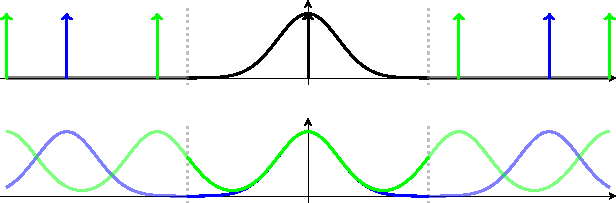
\includegraphics{papers/complex/images/cyclic_conv.pdf}
	\caption{Signal, gefaltet mit Dirac-Folgen unterschiedlicher Periode}
	\label{complex:cyclic-conv}
\end{figure}

Warum dies ein Problem ist, sei mit einem Beispiel illustriert.
In Abbildung~\ref{complex:cyclic-conv} ist ein Beispielsignal, welches mit einem Dirac-Impuls gefaltet werden soll.
Dieser Dirac-Impuls sei nun aber periodisch.
Durch diese Fortsetzung überlappen die verschiedenen Signal-Kopien, falls am Rand nicht extra Platz gelassen wird.
Bei realen Signalen ist dies in der Regel nicht der Fall, die Aufzeichnung beginnt erst, wenn auch etwas Interessantes passiert.

Es ist also wichtig, dem Signal vor der FFT extra Platz einzuräumen, sogenanntes \emph{Signal Padding}.
Dies kann auf verschiedene Arten geschehen.
Abbildung~\ref{complex:padding} zeigt die zwei meistverwendeten, Zero Padding und Spiegeln an den Rändern, am Beispiel einer Cosinus- und Sinus-Schwingung.
\begin{figure}
	\centering
	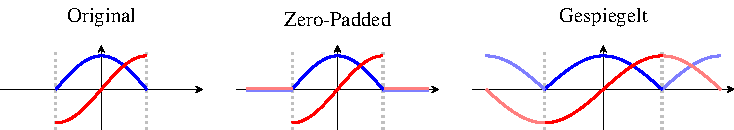
\includegraphics{papers/complex/images/signal_padding.pdf}
	\caption{Verschiedene Signal Padding-Optionen}
	\label{complex:padding}
\end{figure}

Die wohl einfachste Art ist das Ergänzen mit $0$.
Dies führt zu einem Verschwinden des Signals am Rande.
Diese Methode lässt sich gut begründen: kennt man das Signal nicht, nimmt man an, es sei $0$.
Diese Methode ist sicher nie falsch und gibt nur wenig zu tun.

Manchmal kann man das Signal auf geschicktere Art und Weise ergänzen.
Gängig ist etwa, das Signal an den Enden zu spiegeln.
Dadurch bleibt die Intensität des Signals am Rande erhalten.
Sinnvoll ist das jedoch nur, wenn man annehmen kann, dass das Signal auch eine entsprechende Symmetrie aufweist.
Selbst bei einem periodischen Signal tritt dadurch im Allgemeinen eine Unstetigkeit in der Frequenz auf, da die Laufrichtung der Phase invertiert wird.

Anhand der Bilder in Abbildung~\ref{complex:padding} kann man sich leicht überzeugen, dass es keine 'richtige' Art gibt, das Signal zu extrapolieren.
Auch durch Spiegeln des Signals an den Rändern entsteht eine Unstetigkeit, die Frequenz wird invertiert. Dafür tritt kein Phasen-Sprung auf.
Falls die Randwerte wirklich wichtig sind, kann man versuchen, das Signal zu extrapolieren, etwa über eine Polynom-Approximation.
Man sollte sich jedoch im Klaren sein, dass man gerade dabei ist, neue Signal-Werte zu erfinden.

Die Beispielsignale sind so gewählt, dass sie eine ganzzahlige Anzahl Perioden durchlaufen. 
Spiegeln führt dadurch zu einer korrekten Fortsetzung des Signals.
In den bisherigen Bildern wurde diese Methode gewählt, um Artefakte zu vermeiden.
Die Auswirkungen des Signal Paddings können in den Abbildungen~\ref{complex:padding-none}~bis~\ref{complex:padding-sym} betrachtet werden.
\begin{figure}
	\centering
	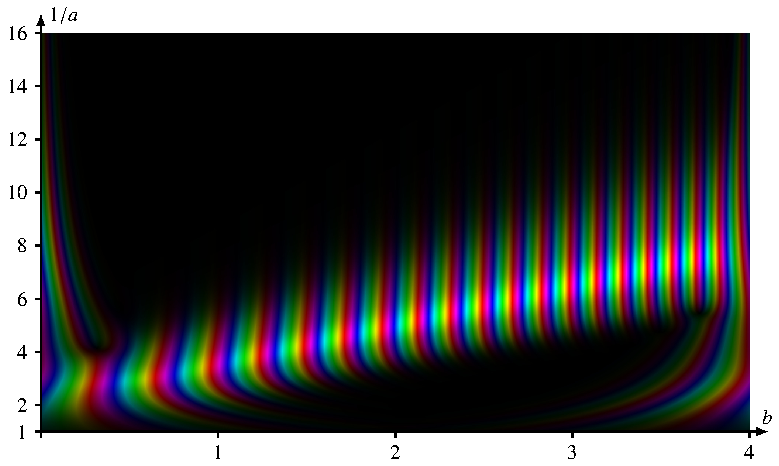
\includegraphics[width=\linewidth, keepaspectratio]{papers/complex/images/padding_none_sweep.pdf}
	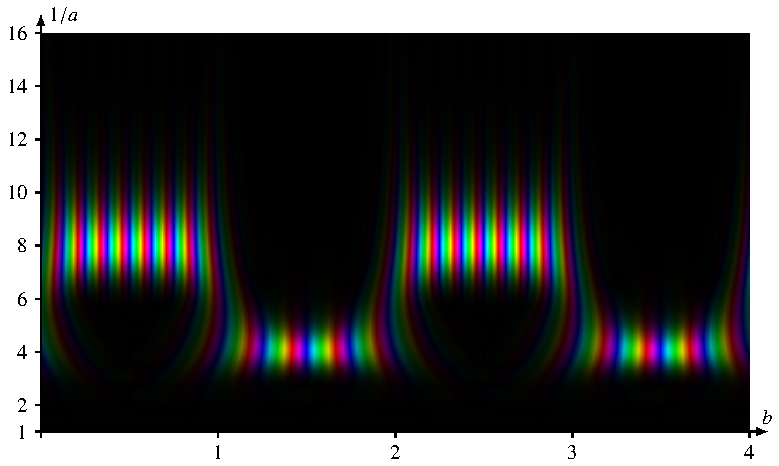
\includegraphics[width=\linewidth, keepaspectratio]{papers/complex/images/padding_none_square.pdf}
	\caption{Ohne Signal Padding. Man beachte, wie die Helligkeit an den Rändern abnimmt. Durch die periodische Fortsetzung entstehen im oberen Bild Artefakte bei ca.~$(0, 7)$ und $(4, 2)$, im unteren bei ca.~$(0,5)$ und $(4,7)$.} \label{complex:padding-none}
\end{figure}

\begin{figure}
	\centering
	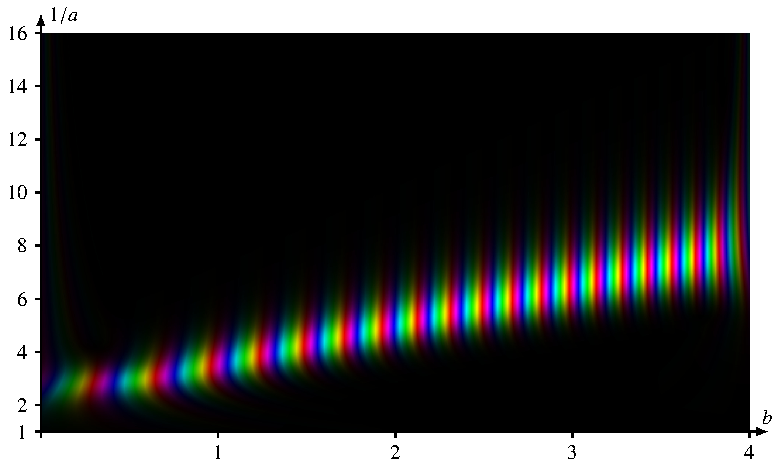
\includegraphics[width=\linewidth, keepaspectratio]{papers/complex/images/padding_zero_sweep.pdf}
	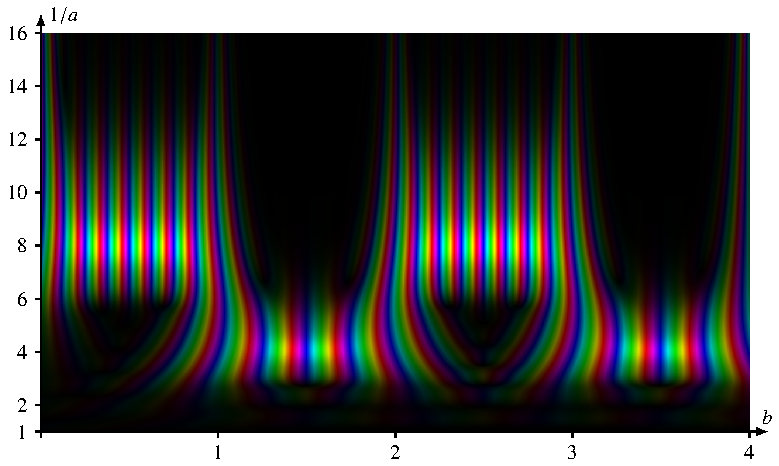
\includegraphics[width=\linewidth, keepaspectratio]{papers/complex/images/padding_zero_square.pdf}
	\caption{Zero Padding. Es sind keine Artefakte erkennbar, aber die Helligkeit an den Rändern nimmt immer noch ab.}
	\label{complex:padding-zero}
\end{figure}

\begin{figure}
	\centering
	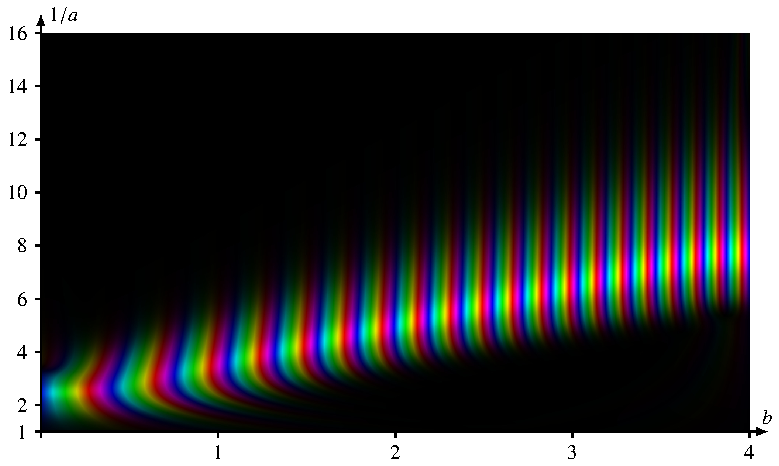
\includegraphics[width=\linewidth, keepaspectratio]{papers/complex/images/padding_sym_sweep.pdf}
	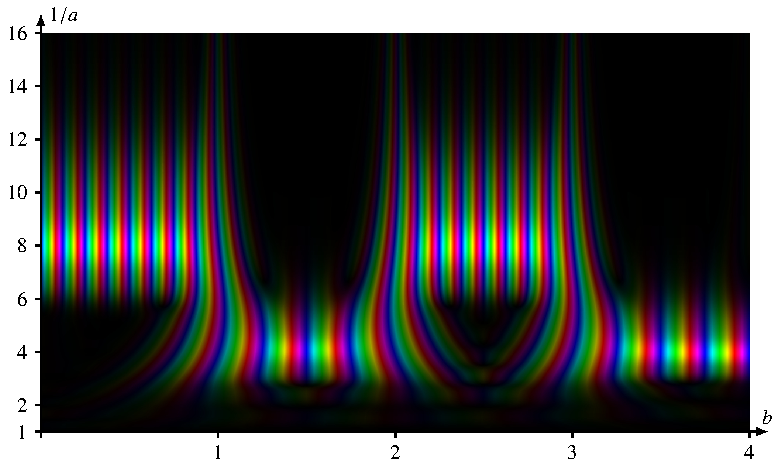
\includegraphics[width=\linewidth, keepaspectratio]{papers/complex/images/padding_sym_square.pdf}
	\caption{Gespiegelt. Es sind keine Artefakte erkennbar und die Helligkeit an den Rändern bleibt erhalten. Man beachte jedoch, dass das hier so gut funktioniert, da die Signale selbst eine klare Periodizität aufweisen und durch Spiegeln quasi perfekt fortgesetzt werden.}
	\label{complex:padding-sym}
\end{figure}

\clearpage